% !TEX encoding = UTF-8
% !TEX TS-program = pdflatex
% !TEX root = ../tesi.tex

%**************************************************************
\chapter{Introduzione}
\label{cap:introduzione}
%**************************************************************

%Introduzione al contesto applicativo.\\
%
%\noindent Esempio di utilizzo di un termine nel glossario \\
%\gls{api}. \\
%
%\noindent Esempio di citazione in linea \\
%\cite{site:agile-manifesto}. \\
%
%\noindent Esempio di citazione nel pie' di pagina \\
%citazione\footcite{womak:lean-thinking} \\

%**************************************************************

\section{Concetti chiave}
\subsection{Processi di business e process mining}
"Il \textbf{processo aziendale} (o business process) è un insieme di attività interrelate, svolte all'interno dell'azienda nell'ambito della gestione operativa delle sue funzioni aziendali, che creano valore trasformando delle risorse (input del processo) in un prodotto finale (output del processo) a valore aggiunto, destinato ad un soggetto interno o esterno all'azienda (cliente)" \cite{site:wiki-business-process}.
\\ 
Un processo è quindi caratterizzato da una sequenza di passi (attività) con lo scopo di raggiungere un obiettivo. \'E importante notare come le varie sequenze sono spesso standardizzate, di conseguenza di avranno, per la maggior parte, esecuzioni simili.
\\ 
A loro volta i processi di business sono la fonte di informazione del process mining. 
\\
"Il \textbf{process mining} è una tecnica di process management, che permette l'analisi dei processi di business basati sui log degli eventi." \cite{site:wiki-process-mining}
\\
Il process mining quindi offre varie tecniche per estrarre informazioni utili dai log degli eventi. Un log di eventi (o \textit{event log}) è una collezione di eventi registrata e tracciata da un sistema informativo conservata in file strutturati (es. CSV, XES, Excel, ecc.) e rappresenta l'impronta digitale elettronica delle varie operazioni aziendali. 
Va osservato che in generale un log va pulito e filtrato prima di poter essere utilizzabile 


\begin{figure}[!h] 
    \centering 
    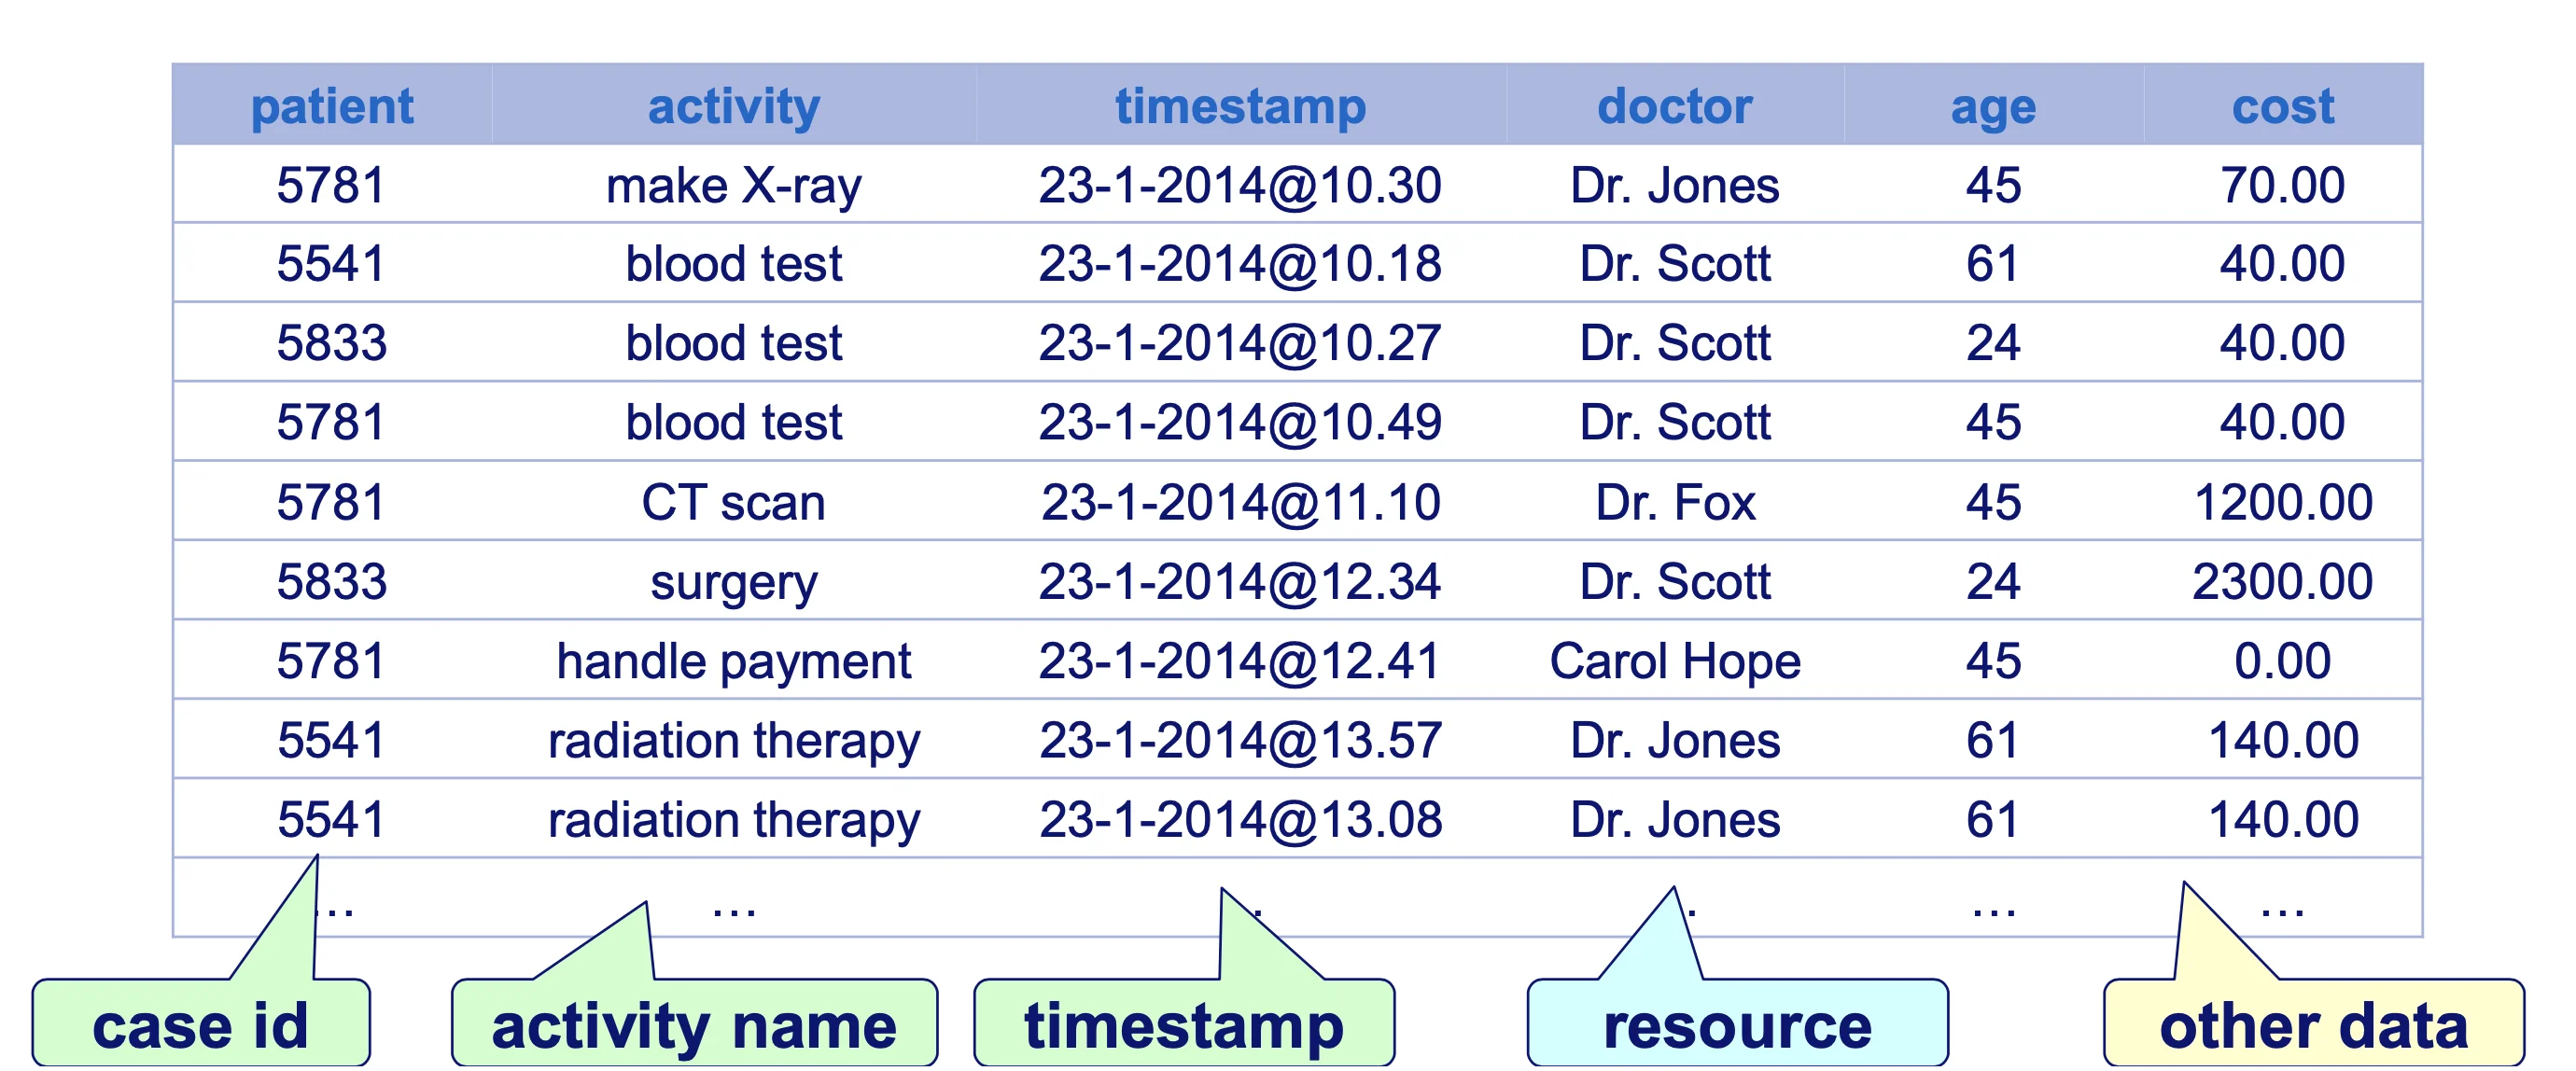
\includegraphics[width=0.9\columnwidth]{immagini/event_log_ex.png} 
    \caption{Esempio di \textit{event log} \cite{site:event-log-img}}
    \label{fig:event-log-img}
\end{figure}


Un evento (osservando la figura \ref{fig:event-log-img}) è una singola "riga" dell'event log, e contiene informazioni relative a:
\begin{itemize}
\item il caso trattato (identificato dal \textit{case id});
\item l'attività eseguita;
\item il riferimento temporale (\textit{timestamp}).
\end{itemize}
Importante notare come i campi appena elencati siano essenziali ed obbligatori, ma un evento può contenere anche altre informazioni aggiuntive (es. risorse, costi, ecc.).
Un insieme di eventi con lo stesso case id viene nominato \textbf{traccia}, quindi un event log può essere visto anche come una collezione di tracce.

Le tecniche di process mining si occupano principalmente di:
\begin{itemize}
\item Process discovery, con lo scopo di generare un \textit{process model}, ovvero una rappresentazione grafica di un processo, permettendone per la visualizzazione, la documentazione e l'estrazione di informazioni;

\item Conformance checking, che confronta il process model con un event log per individuare le differenze e deviazioni, può anche essere utilizzato per valutare la qualità del process model generato durante l'attività di discovery, oppure individuare colli di bottiglia;

\item Enhancement, ovvero il miglioramento del process model attraverso l'introduzione di nuove informazioni (es. misure relative alle performance).
\end{itemize}









